\subsection{Projekt zum Schutz der Biodiversität in Rumänien}

%„schützen durch nutzen“


%Einordnung meiner Arbeit in Relation zum Projekt??? -> Testflüge erwähnen, Zeitrahmen erwähnen???
Das Projekt zum Schutz der Biodiversität in Rumänien ist eine bilaterale Zusammenarbeit im Apuseni-Gebirge zum Erhalt des oligothrophen Grünlandes und insbesondere der Zielart Arnica montana. In zwei Ansätzen soll unter dem Einsatz von moderner Fernerkundungstechnologien einerseits brachliegende Flächen und andererseits Grasland mit Arnica montana erkannt werden. Mit den Erkenntnissen soll auf brachliegenden Probeflächen mit Mäh- und Mulchmaschinen ein Wiesenmanagement stattfinden. Durch die Verwendung von Drohnen sollen bisher unbekannte Flächen mit Arnica montana identifiziert werden, um so mit einer nachhaltigen Arnika-Ernte und Bewirtschaftung die Biodiversität zu erhalten. Das Projekt möchte sich in der Region für Nachhaltigkeit und Naturschutz einsetzten, unter Steigerung des Wohlergehens der lokalen Bevölkerung. 

\subsubsection{Projektpartner}
Das Projekt ist eine Zusammenarbeit der Albert-Ludwigs-Universität Freiburg (ALU-FR) mit dem rumänischen Unternehmen Bioflora Apuseni (BFA) und der Universität für Agrarwissenschaften und Tiermedizin Cluj-Napoca (USAMV). Die ALU-FR wird vertreten durch Prof. Dr. Dr. h.c. Albert Reif (Proffessur für Standort- und Vegetationskunde), Dr. Evelyn Ruşdea  (Projektmanagement) und durch Dr. Holger Weinacker (Institut für Fernerkundung und Landschaftsinformationssysteme). Die ALU-FR hat stellvertretend für das Projekt einen Finanzierungsantrag bei der Deutschen Bundesstiftung Umwelt gestellt.

Das Unternehmen Bioflora Apuseni (BFA) wurde 2010, nach einem langen Prozess der deutsch-rumänischen Zusammenarbeit und Forschung, gegründet. BFA hat es sich zum Ziel gesetzt die ländlichen Bevölkerung im Zentrum des Apuseni Gebirges im nachhaltigen Umgang mit natürlichen Ressourcen zu unterstützten, um die artenreiche Kulturlandschaft der oligotrophen Graslandes zu erhalten und den Lebensstandard zu erhöhen. Das Hauptprodukt ist Arnica montana, welches von den rund 25 SaisonarbeiterInnen von BFA nachhaltig gesammelt und dann in einer lokalen Trocknungsanlage getrocknet. Hauptabnehmer zu einem fairen Preis ist Weleda, die auch gemeinsam mit BFA regelmäßige Schulungen für lokale PflückerInnen organisieren, um die nachhaltige Ernte der Arnikablüten sicherzustellen. Es gibt Entwicklungen? weitere Heilpflanzen zu vermarkten und neue Abnehmer zu finden. Außerdem initiiert BFA weitere Pilotprojekte in anderen Regionen Rumäniens, damit auch dort Arnika nachhaltig geerntet werden kann \citep[vgl.][]{ECOKARST2018,DBU2018}.

Die Universität in Cluj-Napoca (USAMV) erforscht seit 2000 im Apuseni Gebirge die traditionelle Bewirtschaftung des Graslandes, um das Management zu optimieren und zu erhalten. Es gibt unter anderem eine Langzeitstudie zu den Folgen von Düngern auf die Biodiversität des Graslandes im Apuseni Gebirge. Als assoziierter Partner wird der Drohnen-Pilot und Videoeditor Paul Crişan für das Projekt an der USAMV angestellt. Weitere assoziierte Partner sind der Naturpark Apuseni, die LEADER-Initiative (GAL Arieşul Mare) sowie die Firma Weleda.

Bereits von 2000 bis 2004 gab es eine erste Zusammenarbeit der ALU-FR mit der rumänischen USAMV mit dem gemeinsamen „Projekt Apuseni“, aus dem die Identifizierung von Arnica montana im Zentrum des Apuseni Gebirges hervorging. Finanziert durch das Bundesministerium für Bildung und Forschung (BMBF) wurden sieben kleinere Pilotprojekte in verschiedenen Bereichen, wie ländlichem Tourismus, Landwirtschaft, Wasserversorgung, Arzneipflanzen und Waldwirtschaft durchgeführt. Dabei wurde bewusst ein partizipativer Ansatz (buttom-up) gewählt, da vor Ort die Landschaft Allgemeingut ist, das von vielen Menschen beansprucht wird. Deshalb wurden auch möglichst viele Personen in den Prozess der Entwicklung eines nachhaltigen Landschaftmanagements involviert. Neben Interviews mit LandwirtInnen, ExpertInnen und lokalen PolitikerInnen wurden Treffen, Workshops und  Vorträge organisiert, Informationsmaterialien verteilt, Beratungen und Rollenspiel durchgeführt und ein Schul-Projekt „Planning for real“ angeboten. Darin bauten die SchülerInnen gemeinsam ein dreidimensionales Modell des Dorfes, wie es in 15 Jahren aussehen soll. Aus den Projekten ließen sich die Stärken und Schwächen der Bergregion herausfiltern, um damit Empfehlungen für die regionale Entwicklung zu formulieren? \citep[vgl.][]{RUSDEA2009}.
Im Anschluss startete ein weiteres Projekt, diesmal mit dem Schwerpunkt auf \textit{Arnica montana}, 2004 im Apuseni Gebirge. Das „Arnika Projekt“ lief bis 2007 und wurde vom World Wide Fund For Nature (WWF) und der Darwin Foundation is Zusammenarbeit mit der USAMV durchgeführt. Im Ausbau der Kooperation mit der lokalen Bevölkerung wurde der Kontakt zu BesitzerInnen von oligotrophen Wiesen und potenziellen Arnika PflückerInnen hergestellt. Durch Interviews wurde die traditionelle Bewirtschaftung der oligotrophen Wiesen erforscht und Trainings zur nachhaltigen Ernte der Blütenstände der \textit{Arnica montana} durchgeführt \citep[vgl.][20]{DBU2018}.

\begin{figure}[htb]
 \centering
 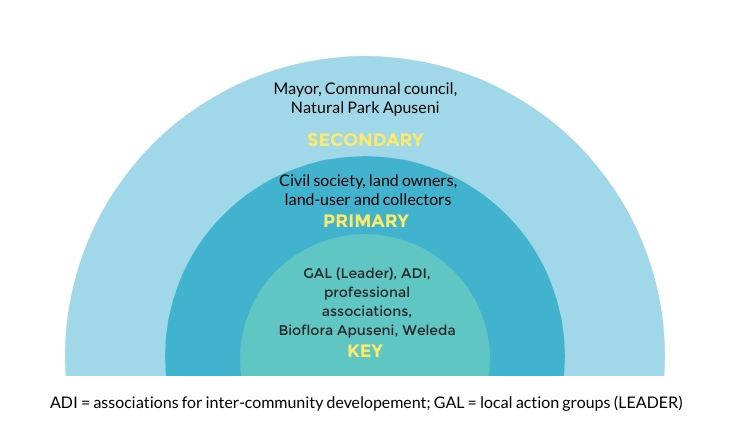
\includegraphics[width=0.7\textwidth,angle=0]{abb/Stakeholder-map}
 \caption{Stakeholder map \citep[In Anlehnung an][]{DBU2018}}
\label{fig:stakeholdermap}
\end{figure}

%Stakeholder map erklären:
Im Projekt wird zwischen Key Stakeholder, primären und sekundären Stakeholdern unterschieden (Siehe Abbildung~\ref{fig:stakeholdermap}, S.\pageref{fig:stakeholdermap}). Die etablierten Organisationen, wie BFA, Weleda und die lokale Aktionsgruppe (LAG/GAL) Arieşul Mare und die Associations for inter-community development (ADI) sind aufgrund von ihrer Erfahrung im Naturschutz vor Ort die Key Stakeholder. Primärer Stakeholder ist die ansässige Bevölkerung, insbesondere die EigentümerInnen oder PächterInnen der Flächen oder SammlerInnen der Wildkräuter. Als sekundäre Stakeholder bilden die die administrativen Stellen in der lokalen und regionalen Behörden und die Verwaltung des Naturparks Apuseni.

\subsubsection{Ökologischer Hintergrund}

Das Apuseni Gebirge befindet sich im nordwestlichen Teil von Siebenbürgen in Rumänien. Es bildet den nördlichen Teil der Rumänischen Westkarpaten und erreicht Gipfelhöhen von 1100 bis 1800 m. Die Landschaft ist geprägt durch Steilhänge und Karstformen, wie Dolinen, Polje, Trockentälern, Karsttreppen und Unterirdischen Höhlen. Die Region hat eine geringe Einwohnerdichte, aber die höchste Einwohnerdichte im Vergleich zu anderen Bergregionen Rumäniens. Vor einer Besiedelung gab es ursprünglich nur Waldgebiet mit Kiefer und Buchen. Durch die Nutzung der Ressource Holz entstand das Grasland von heute. Die Landnutzung beträgt heute noch ca. 55\% Wald (davon ca. 79\% Laubwald, 12,34\% Nadelwald und 3,5\% Mischwald, Rest ist Übergangsvegetation), 17,4\% Grasland, 3,09\% Brachland, 1,84\% Besiedelung und 0,61\% Ackerland (Gärten).

Vor 1989 war die Waldwirtschaft in Rumänien streng geregelt und kontrolliert. In der Zeit danach nahm die Walddegradation und Entwaldung im Apuseni Gebirge stetig zu, weil der kommerzielle Vermarktung von Holz europaweit als wirtschaftlich rentable erkannt wurde. Dies führte zum drastischen Rückgang der Wälder im Apuseni-Gebirge, insbesondere von Nadelbäumen. Die derzeitige Regierung versucht dem entgegen zu wirken und hat neue Regelungen erlassen, nach denen pro Person nur 20m\textsuperscript{3} Holz im Jahr gefällt werden dürfen. Größere Unternehmen sind davon ausgenommen, was einen Nachteil für die lokalen Bevölkerung darstellt, die ihre Haupteinnahmequelle, die Holzverarbeitung und Aufwertung, verliert. Eine signifikante Abwanderung ist die Folge, was auch einen negativen Effekt auf das Management von Grasland hat.

\begin{figure}[htb]
 \centering
  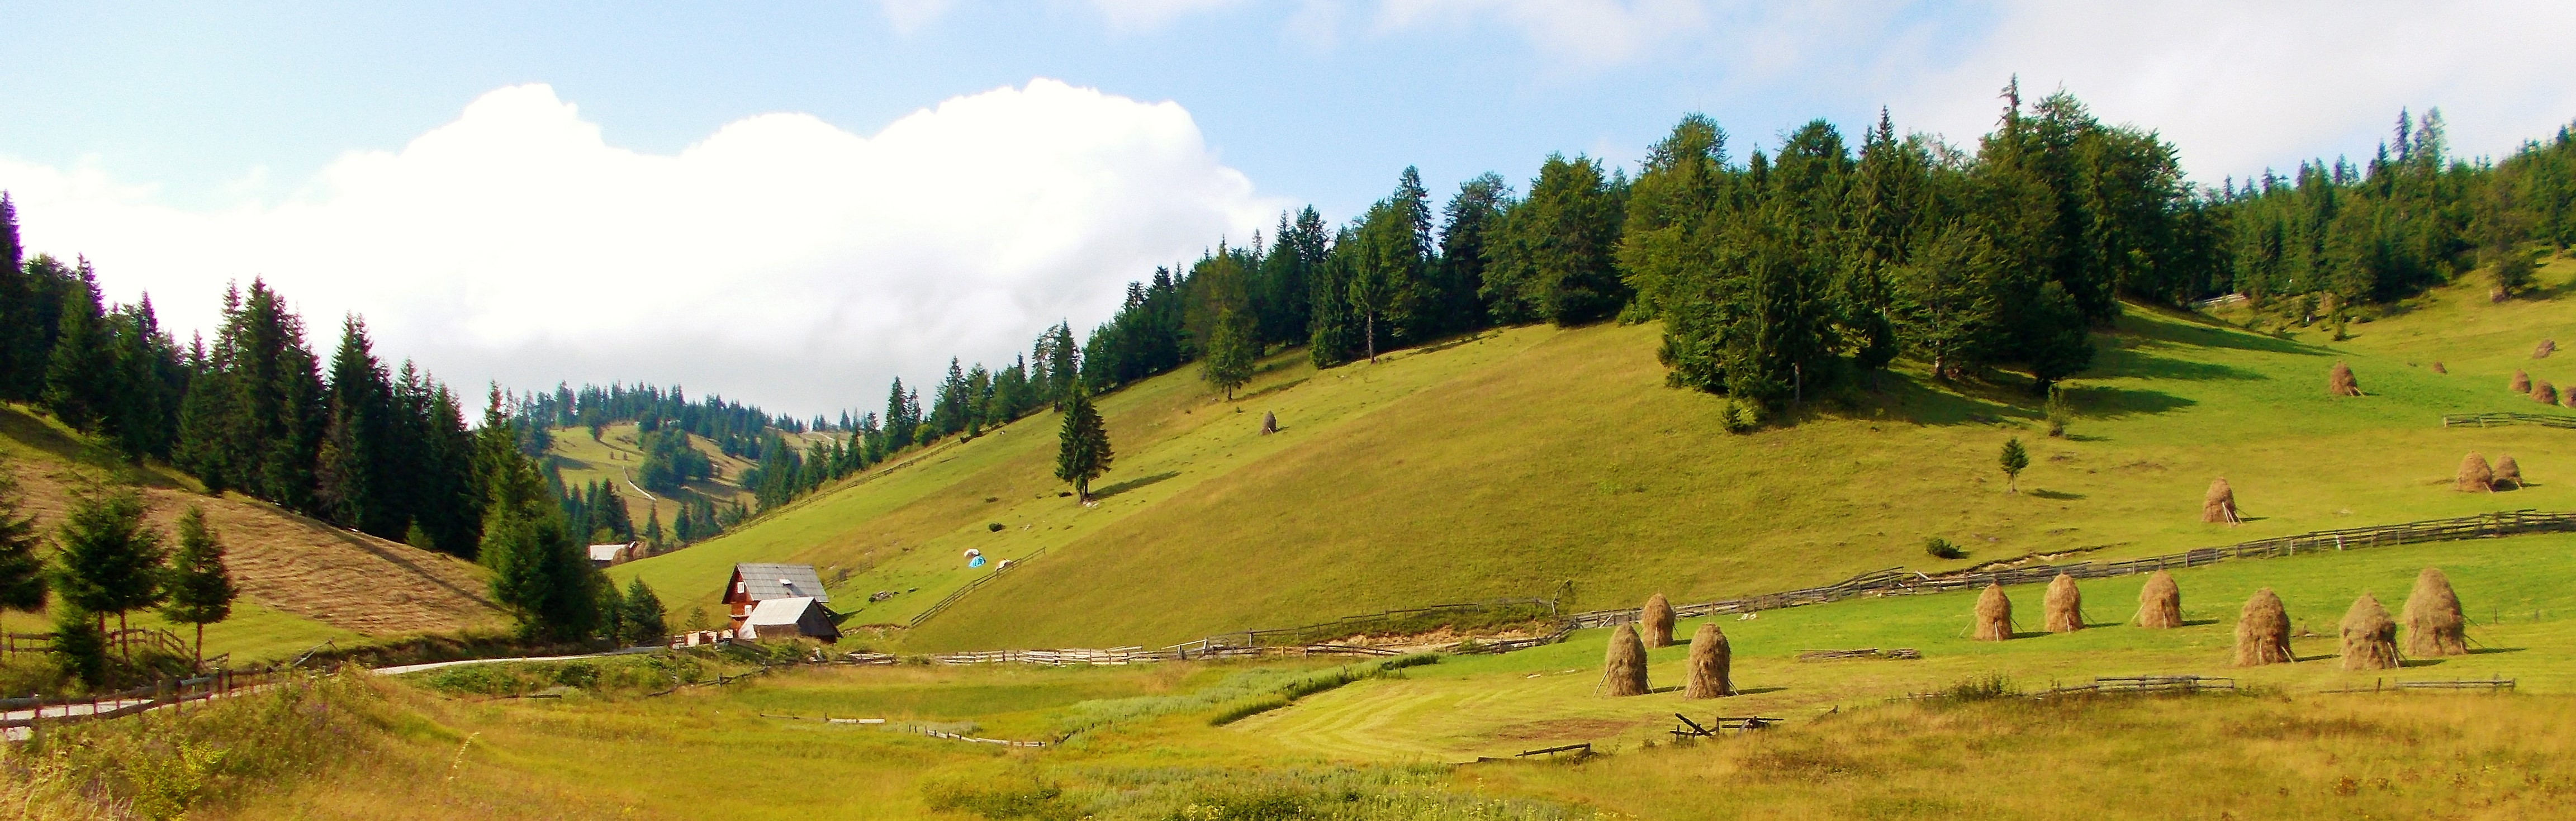
\includegraphics[width=\textwidth,angle=0]{abb/Arnika/apusenimountain2016}
 \caption{Apuseni Gebirge mit traditioneller Heuernte \citep{Farcas2019}}
\label{fig:apuseni}
\end{figure}

Das oligotrophe Grasland kann seine Biodiversität nur erhalten, wenn eine Bewirtschaftung stattfindet. Das Brachliegen oder die Intensivierung der Nutzung gefährdet das schwierige Gleichgewicht der Graslandwiesen. Zum Schutz der Biodiversität muss eine gemäßigte Düngung von biologischen Düngern (keine Mineraldüngung!) periodisch aufgetragen werden. Um optimale Bedingungen für eine hohe Vielfalt an Arznei- und Wildpflanzen zu erhalten, müssen die Flächen etwa jährlich gemäht werden und dazwischen geflegt werden, z.B. durch das Entfernen von Ästen und Steinen.

\tg{hier muss noch zu dem tatsächlichen Manangement recherchiert werden}

\subsubsection{Vorgehensweise}

Der Projektzeitplan sieht einen Start ab dem Frühjahr 2019 vor und das Projekt soll über einen Zeitraum von drei Jahren laufen. Jährlich im Juni/Juli sollen die Drohnenflüge zur Identifizierung von Arnika stattfinden. Im September/Oktober werden die Grasland-Flächen beflogen, um eine Bewirtschaftung oder das brachliegen festzustellen. Zur Vorbereitung auf die Datenerhebungen in Rumänien fanden im Juli 2018 Drohnenflüge zu Testzwecken im Schwarzwald statt.

Zur Identifikation von brachliegendem oligotrophen Grasland sollen mit dem Einsatz von Drohnen Digitale Höhenmodelle erstellt werden. Dafür muss das gesamte Gelände zweimal mit der Drohne erfasst werden. Beim ersten Flug wird ein Digitales Oberflächen Modell (DOM) (engl. digital surface model DSM) erstellt, also ein Modell der Erdoberfläche inklusive auf ihr befindlicher Objekte, wie die Vegetation. Nach dem zweiten Flug kann ein Digitales Geländemodell (DGM) (engl. digital terrain model DTM) abgeleitet werden. Das DGM ist ein Modell der natürlichen Erdoberfläche ohne Objekte. Durch die Subtraktion der beiden Modelle kann ermittelt werden, ob Flächen gemäht wurden oder ob sie brachliegen. Nach der Indentifikation von brachliegenden Flächen werden fünf Probeflächen in fünf Gemeinden ausgewählt und durch den Einsatz von Mäh- und Mulchmaschinen wieder nutzbar gemacht. In Zusammenarbeit mit der lokalen Aktionsgruppe Arieşul Mare soll der Kontakt zwischen LandbesitzerInnen initiiert werden. Mit dem Zusammenschluss gibt es die Perspektive weitere Technologien und Maschinen anschaffen zu können und das Projekt auf andere Regionen ausweiten zu können.

Mit der nachhaltigen Vermarktung von Arnica montana soll in die Bevölkerung ein Interesse zum Schutz des oligotrophen Graslandes geschaffen werden. Durch die Verknüpfung der ökonomischen Interessen mit dem ökologischen Erhalt der Biodiversität soll langfristig eine Steigerung der Lebensqualität der vor Ort lebenden Menschen erreicht werden. An die Entwicklung der BFA soll hier angeschlossen werden. Ziel ist es eine Datenbank und Karte über die Verteilung der Arnika-Flächen in zehn Gemeinden zu erstellen. Durch den Einsatz von Drohnen in fünf Gemeinden soll das Produktivitätspotential der Habitate ermittelt und in eine qualitative Klasse in Abhängigkeit von der Anzahl der Blütenstände pro 100 m\textsuperscript{2} eingeordnet werden. Zusätzlich soll erfasst werden, welches Management bisher auf den Flächen durchgeführt wurde. Für die Auswertung der durch den Drohneneinsatz entstandenen Bilder soll ein Software-Programm entwickelt werden, dass die Arnica montana Blütenstände automatisch erkennt und eine Klassifizierung durchführt.

\subsection{Drohneneinsatz zur Fernerkundung}

%+++ Was ist eine Drohne? Was eine UAS, UAV?
Drohnen sind Luftfahrzeuge, die ohne an Bord befindliche Personen über einen Computer oder vom Boden aus über eine Fernsteuerung betrieben werden. Unbemannte Luftfahrzeuge (engl. Unmanned Aerial Vehicle, kurz UAV) besitzen zwei Tragflächen und sind dem Flugzeug nachempfunden. Multikopter zählen zu den Hubschraubern und haben zwischen zwei und zwölf Rotoren, so können sie sich in alle Richtungen bewegen. Beide werden im allgemeinen Sprachgebrauch Drohnen genannt. Ferngesteuerte Fluggeräte, die im Freizeitbereich eingesetzt werden, zählen nicht zu den Drohnen, auch wenn vor allem die Multikopter Flugmodelle oft so bezeichnet werden. Unmanned Aerial Systems (UAS) bestehen aus der UAV, der Sensor-Ladung und der Bodenkontrollstation. Komponenten und Größe der Bodenkontrollstationen variieren stark, in Abhängigkeit von der Aufgabe der UAV. Sie können aus großen Kontrollsystemen bestehen, die auf Fahrzeugen montiert werden oder nur aus einem kleinen Laptop, der getragen werden kann. Die Klassifizierung von UAS im zivilen wissenschaftlichen Einsatz orientiert sich generell auf den schon vorhandenen militärischen Begriffen. Die Einteilung basiert auf den Eigenschaften Größe, Flugausdauer und weiteren Fähigkeiten der Drohnen \citep[vgl.][]{Watts2012}.

\subsubsection{Vergleich von Drohnenarten}

Für den Anwendungsmaßstab des Projekts in Rumänien sind zwei Arten von Drohnen geeignet (Siehe Abbildung~\ref{fig:drohnen}, S.\pageref{fig:drohnen}). Die Multikopterdrohnen können präzise Aufnahmen in einer angemessene Höhe machen, haben durch den Schwebflug aber einen höheren Energieverbrauch und somit eine kürzere Flugdauer. „Vertical Take-Off and Landing“ (VTOL) Drohnen sind UAV, die keine Start- oder Landebahn benötigen. Durch ihre Tragfläche können VTOL Drohnen eine große Fläche in geringer Zeit befliegen. Zum Starten und Laden haben sie Rotoren, die nach oben gerichtet werden. Dadurch sind sie auch in unwegsamen Gelände einsetzbar.
Generell stehen die mögliche Flugzeit und damit auch die Größe der Fläche, die von der Drohne erfasst werden kann, in Abhängigkeit zum Gewicht der Drohne. Eine höhere Beladung, durch weitere Sensoren, beispielsweise eine Kamera mit einem größerem und schwerem Objektiv, bringen genauere Ergebnisse, aber verkürzen durch ihr Gewicht die mögliche Flugzeit. Einen großen Teil des Gewichts macht aber auch der Akku aus, dessen Größe sich aber auch positiv auf die Flugdauer auswirkt.

\begin{figure}[hbt]
    %\hspace{-20pt}
    \subfigure{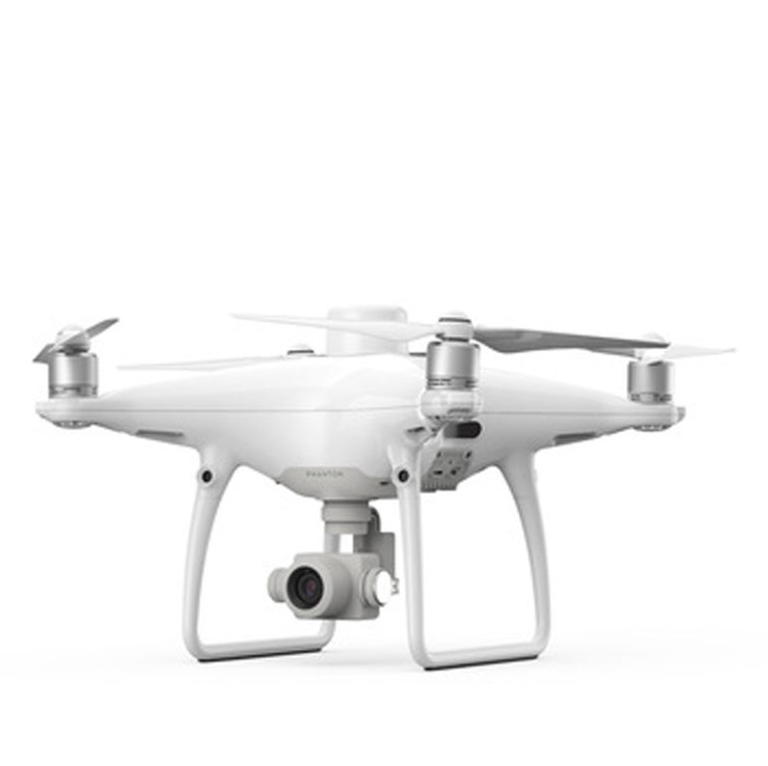
\includegraphics[width=0.20\textwidth]{abb/drohnen/P4RTK}}
    \hspace{-20pt}
    \subfigure{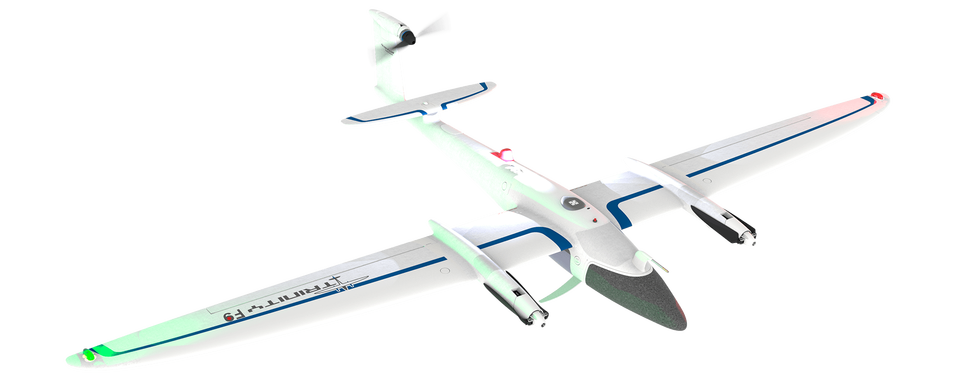
\includegraphics[width=0.52\textwidth]{abb/drohnen/trinity-f9}}
        \hspace{-30pt}
    \subfigure{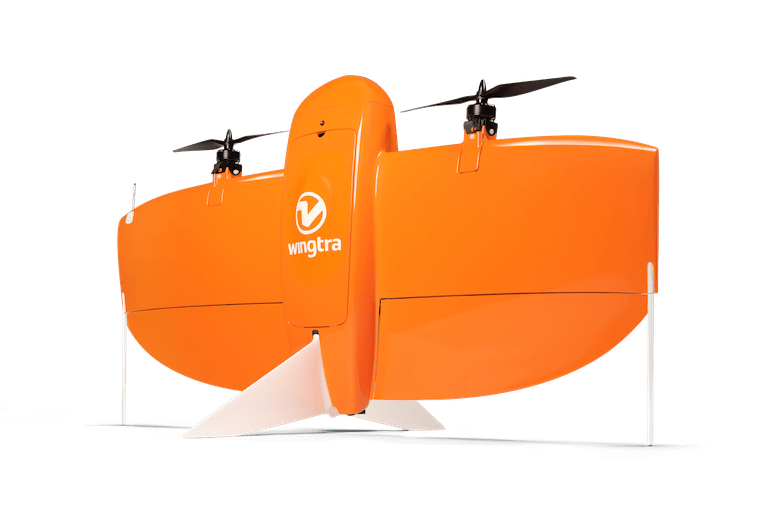
\includegraphics[width=0.35\textwidth]{abb/drohnen/wingtraone}}
     \hspace{-20pt}
\caption{ v.l.n.r: DJI Phantom 4 Quadrocopter \citep{DJI2019}, Trinity F9 \citep{QSGH2019} und WintraOne VTOL-Drohnen \citep{Wingtra2019}}
     \hspace{-40pt}
  \label{fig:drohnen}
\end{figure}

Das „Projekt zum Schutz der Biodiversität in Rumänien“ behandelt zwei Aufgaben, die unterschiedliche Anforderungen an eine Drohne stellen. Bei der Befliegung des Graslandes zur Erkennung von brachliegenden Flächen ist eine riesige Fläche zu erfassen. Eine UAV mit Starrflügeln kann im Vergleich zu Multikoptern höher fliegen und hat somit eine größere Flugausdauer, so kann eine größere Fläche abdeckt werden. Mit einer „Vertical Take Off and Landing“ Drohne (VTOL) können Schäden beim Start oder Ladung in unebenen Gelände vermieden werden. Da die Vegetation des Graslandes nur eine Höhe von 20-30 cm hat, muss zur genauen Berechnung der Höhenmodelle die möglichst genaue vertikale und horizontale Position der Drohne erfasst werden. Dementsprechend wird ein System  benötigt, dass die Ungenauigkeiten der globalen Navigationssysteme (GNSS), die üblicherweise ein paar Meter betragen, ausgleicht. Mit real-time kinematics (RTK) und post-processing kinematics (PPK) Systemen kann eine genaue Positionsbestimmung bis auf wenige Zentimeter berechnet werden. Wie der Name schon sagt, findet diese Berechnung beim RTK in unmittelbar statt, beim PPK nachgelagert. 
Der Vorteil von RTK und PPK ist, dass die Verwendung von Bodenreferenzpunkten entfällt, was Kosten spart. Für Beide wird eine GNSS-Bodenstation benötigt, die georeferenziert ist, um ein genaues Ergebnis zu erzielen. Bei PPK kann auch falls vorhanden mit einer virtuellen Referenzstation gearbeitet werden. Bei RTK muss eine Verbindung zwischen Drohne und GNSS-Bodenstation vorhanden sein, bei Störungen kann ein genaues Ergebnis nicht berechnet werden. Bei PPK ist eine Verbindung nicht notwendig, die genaue Positionierung wird erst bei Auswertung der Log-Daten berechnet. 

Für die Identifizierung von 5-8 cm großen Arnika-Blüten benötigt man hingegen eine Drohne, die Bilder in einer möglichst hohen Auflösung machen kann. Da Starrflügel UAVs eine höhere Mindestgeschwindigkeit haben als Multikopter, die auch in der Luft „stehen“ können, könnte sich die Fluggeschwindigkeit negativ auf die Qualität der Bilder auswirken. Einerseits sollen großflächige Befliegungen Flächen mit Arnica montana lokalisieren, um das Monitoring auszuweiten. Andererseits soll eine qualitative Analyse der Flächen stattfinden. Für die großflächige Befliegung eignet sich eine VTOL-Drohne, die eine möglichst hohe Auflösung erzielt dabei aber eine große Fläche befliegen kann. Für die qualitative Analyse der Flächen kann noch höhere Auflösung nötig sein, die durch eine tiefere Flughöhe mit geringer Geschwindigkeit erreicht werden. Mit einem Multikopter kann dies ohne große Umstände passieren.

\begin{table}[hbt]
\fontfamily{cmss}\selectfont
\footnotesize
\begin{tabular}{lccc} %\toprule
\textbf{Technische Daten} & \textbf{DJI Phantom 4 RTK} & \textbf{Trinity F9}  & \textbf{WingtraOne} \\ %\midrule
\hline\hline
Flügelbreite & 0,35 m & 2,394 m & 1,25 m \\
Max. Startgewicht & 1,391 kg & 4,5 kg & 4,5 kg \\
max. Zuladung & – & 550 g & 800 g \\
Fluggeschwindigkeit & max 50 – 58 km/h & 60 km/h & 57,6 km/h \\
Max. Flugzeit & 30 min & 60 min & 55 min \\
Windwiderstand am Boden & 10 m/s & 7 m/s & 8 m/s \\
Windwiderstand im Flug & 10 m/s & 12 m/s & 12 m/s \\
Max. Fläche & 100 ha (182 m) & 500 ha (100 m) & 320 ha (120 m) \\
Auflösung & 1,5 cm/px (120 m) & 2,5 cm/px (100 m) & 2,8 cm/px (120 m) \\
Sensoren & RTK und Gimbal\textsuperscript{1} & PKK & PKK \\
Positionierungsgenauigkeit\textsuperscript{2} &  & 2 – 5 cm &  \\
{    } vertikal & 1,5 cm + 1 ppm RMS &  & 2 cm  \\
{    } horizontal & 1 cm + 1 ppm RMS &  & 1 cm + 0,003\% RMS\\
Preis & ca. 7.800 EUR & ca. 14.850 EUR & ca. 36.678 EUR\\
\hline
\end{tabular}
\\
\scriptsize
1: Gimbal ist ein Bildstabilisator \\
2: RMS = Root Mean Square entspricht der Standardabweichung \\
1 ppm = pro km nimmt Wertgenauigkeit um 1 mm ab. 
\caption{Technische Daten der Drohnen im Vergleich \citep[vgl.][]{DJI2019,QSGH2019,Wingtra2019}}
\label{tab:technischedaten}
\end{table}

Derzeit gibt es eine Vielzahl von Drohnen in allen Preissegmenten zum privaten und wissenschaftlichen Gebrauch auf dem Markt. Drei Vertreter, die für die Aufgaben des Projektes in Rumänien in Frage kommen würden, sind der Quadrocopter DJI Phantom 4 RTK, die VTOL-Drohne Trinity F9 von Quantum-Systems und die VTOL-Drohne WintraOne PPK. Ausgewählt wurden diese weil sie alle ein System zur Positionskorrektur (PPK oder RTK) besitzen. Dies ist notwendig, um genaue digitale Höhenmodelle zu berechnen. Schaut man sich die drei Drohnen an (Siehe Abbildung~\ref{fig:drohnen}, S.\pageref{fig:drohnen}), fallen zunächst die großen äußeren Unterschiede auf. Mit einer Flügelbreite von über 2 m ist die Trinity F9 die größte Drohne. Die WingtraOne ist für eine Starrflügel Drohne mit einer Flügelbreite von nur 1,25 m recht klein. Trotzdem sind beide VTOL-Drohnen, können also aus dem Stand starten. Die Trinity F9 dreht dafür ihre Rotoren nach oben und schwebt waagerecht in die Luft, vergleichbar mit einem Multikopter. Die WintraOne starten senkrecht in die Luft und dreht dann in gewünschter Höhe den Flugkörper. Vergleicht man die Technischen Daten der Drohnen (Siehe Tabelle~\ref{tab:technischedaten}, S.\pageref{tab:technischedaten}) unterscheiden sie sich im Windwiderstand, also die maximale Windgeschwindigkeit bei der mit den Drohnen geflogen werden sollte, nur geringfügig. Auch bei der Fluggeschwindigkeit scheint es nur minimale Unterschiede zu geben, allerdings ist dies bei der DJI Phantom 4 RTK die maximale Fluggeschwindigkeit, der Quadrocopter kann durchaus auch wesentlich langsamer fliegen und damit genauere Bilder aufnehmen. Bei den VTOL-Drohnen ist die angegebene Fluggeschwindigkeit die „cruise speed“ also durchschnittliche Fluggeschwindigkeit im aerodynamischen Flug, ein wesentlich geringere Fluggeschwindigkeit ist nicht möglich. Der Quadrocopter unterscheidet sich im Vergleich zu den beiden VTOL-Drohnen wesentlich in Größe, Gewicht und Zuladungsmöglichkeit. Die DJI Phantom 4 RTK Drohne wiegt nur 1391 g Größe von nur 35 cm in der Diagonale. Eine zusätzliche Zuladung ist nicht möglich, die Kamera und Sensoren sind integriert. Trotz des wesentlich geringerem Gewichts der Drohne kann sie nur etwa 30 min fliegen und damit etwa halb so lang, wie die VTOL-Drohnen. Die Fläche die von der Drohne erfasst werden kann, ist dementsprechend auch wesentlich geringer, nur 100 ha bei einer Flughöhe von 182 m. Mit der WingtraOne Drohne kann eine Fläche von 320 ha bei 120 m Flughöhe erfasst werden, mit der Trinity F9 sogar 500 ha bei 100 m Flughöhe. Allerdings haben die Bilder, die bei der Flughöhe von den VTOL-Drohnen gemacht werden nur eine Auflösung von 2,5 cm/px (Trinity F9 bei 100 m) bis 2,8 cm/px (WingtraOne bei 120m). Die DJI Phantom 4 RTK schafft bei 120 m Flughöhe eine deutlich bessere Auflösung mit 1,5 cm/px. Ein weiterer entscheidener Unterschied besteht in der Positionierungsgenauigkeit. Die DJI Phantom 4 RTK und die WingtraOne PKK erreichen eine Genauigkeit von etwa 1 bis 2 cm. Die Trinity F9 erreicht mit ihrem PKK System nur eine Positionsgenauigkeit von 2 bis 5 cm. Dies ist, neben dem Preis, der entscheidenste Unterschied zwischen den beiden VTOL-Drohnen WingtraOne und Trinity F9. Preislich ist der Quadrocopter am günstigsten mit 7800 Euro. Die Trinity F9 Drohne ist für etwa 14850 Euro erhältlich und die WingtraOne kostet 36678 Euro. %-> Ein Vorteil der DJI Phantom 4 RTK ist auch noch das Ausweichsystem, ???
Für die Aufgabe der Erfassung von brachliegenden Flächen im „Projekts zum Schutz der Biodiversität in Rumänien“ sind die Trinity F9 und die WingtraOne Drohne geeignet. Allerdings können bei der Berechnung der digitalen Höhenmodelle mit der Trinity F9 aufgrund von der geringeren Positionierungsgenauigkeit Fehler entstehen. Die WingtraOne hat dort einen entscheidenen Vorteil. Für die Erkennung von Arnica montana könnte mit einer VTOL-Drohne ein größeres Gelände beflogen werden, um einen Hinweis auf Arnica montana zu geben, für eine präzise qualitative Analyse könnten mit der DJI Phantom 4 RTK gute Ergebnisse erzielt werden. Eine Drohne, die für beide Aufgaben mit besten Ergebnissen verwendet werden kann, ist die WingtraOne. Mit einer geringen Flughöhe und einer lichtempfindlichen Kamera kann auch die WingtraOne Bilder mit einer Auflösung machen, die eine qualitative Analyse von Arnikablüten möglich macht. 

\subsubsection{Testflüge im Schwarzwald}
%++++++ Testflüge?? im Schwarzwald 

Bei Testflügen im Schwarzwald im Juli 2018 wurden erste Bilder an einem bekannten Standort von Arnica montana gemacht. Mit der Octocopter-Drohne der Universität Freiburg wurden mit einer Sony Alpha 7R Kamera eine Fläche in unterschiedlichen Flughöhen erfasst. 
\begin{wrapfigure}{r}{0.4\textwidth}
  \vspace{-30pt}
  \begin{center}
    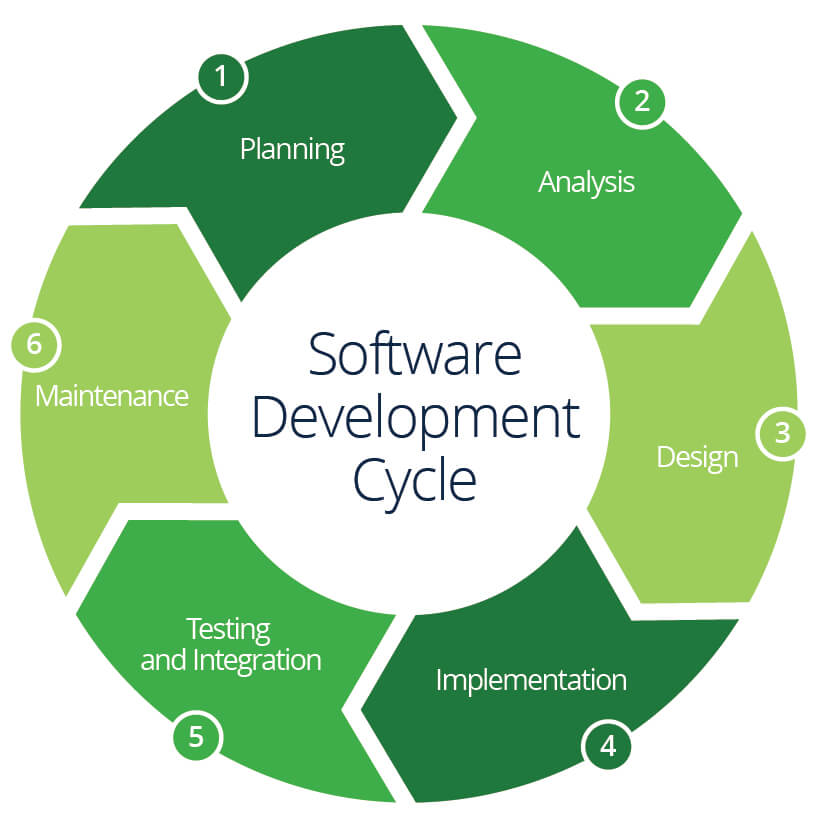
\includegraphics[width=0.4\textwidth]{abb/SDLC}
  \end{center}
  \vspace{-20pt}
  \caption[System Developement Life Circle \citep{Smartsheet2019}]{\footnotesize SDLC \citep{Smartsheet2019}}
  \label{fig:sdlc}
  \vspace{-20pt}
\end{wrapfigure}

Anschließend wurden die Daten ausgewertet, Höhenmodelle berechnet und Orthofotos erstellt. Ziel war es mit den Testflügen den Bedarf und Beschaffenheit der Ausrüstung für die spezifische Aufgabe heraus zu finden. Mit den entstandenen Testdaten sollen erste Methoden? entwickelt werden und damit der System Developement Life Circle (SDLC) in Gang gesetzt (Siehe Abbildung~\ref{fig:sdlc}, S.\pageref{fig:sdlc}). Die Softwareentwicklung durchläuft verschiedene Phasen, die aufeinander aufbauen. Im Laufe der Entwicklung können sich die Phasen im Kreislauf wiederholen, um Änderungen einzuarbeiten und Fehler auszubessern. 

\begin{table}[hbt]
\fontfamily{cmss}\selectfont
\begin{tabular}{lcccc} %\toprule
\textbf{} & \textbf{Flug 1} & \textbf{Flug 2}  & \textbf{Flug 3} & \textbf{Flug 4} \\ %\midrule
\hline\hline
Flughöhe & 13,8 m & 20,3 m & 27,8 m & 64,6 m \\
Anzahl Bilder & 236 & 208 & 233 & 355 \\
Auflösung am Boden & 1,32 mm/px & 1,89 mm/px & 2,6 mm/px & 5,93 mm/px \\
Erfasste Fläche & 1.04e+03 m\textsuperscript{2} & 633 m\textsuperscript{2} & 950 m\textsuperscript{2} & 0.0174 km\textsuperscript{2} \\
\hline
\end{tabular}
\caption{Technische Daten? der Testflüge}
\label{tab:flugvergleich}
\end{table}

Die vier Flüge sollten in der Höhe von 15 m, 20 m, 30 m und 80 m Aufnahmen machen, um Bilder mit unterschiedlicher Auflösung für die Softwareentwicklung zu haben. Die tatsächliche Flughöhen lassen sich der Tabelle~\ref{tab:flugvergleich} auf S.\pageref{tab:flugvergleich} entnehmen. Gerade beim letzten Flug, weicht die tatsächliche Flughöhe erheblich von der geplanten ab. Auch die Lichtverhältnisse sind bei Flügen sehr unterschiedlich und deutlich auf den Aufnahmen erkennbar (Siehe Abbildung~\ref{fig:gleicheblumen} und \ref{fig:gleicherausschnitt}, S.\pageref{fig:gleicheblumen}. Bei den ersten beiden Flügen in etwa 15 m und 20 m sind die Blüten noch sehr gut erkennbar. Bei den Aufnahmen aus ca. 30 m und 80 m (tatsächlich etwa 65 m) Flughöhe wird die Bildqualität zunehmend schlechter. Die Auflösung beträgt bei 65 m Höhe auf dem Boden nur noch etwa 0,6 cm/px. Das Bild ist sehr unscharf und die Blumen sind nur noch als gelbe Punkte erkennbar. 

\begin{figure}[htb]
    \subfigure[Flug 1]{\includegraphics[width=0.24\textwidth]{abb/ergebnisse/gleicherausschnitt/DSC01525-a}}
    \subfigure[Flug 2]{\includegraphics[width=0.24\textwidth]{abb/ergebnisse/gleicherausschnitt/DSC01298-a}}
    \subfigure[Flug 3]{\includegraphics[width=0.24\textwidth]{abb/ergebnisse/gleicherausschnitt/DSC01757-a}}
    \subfigure[Flug 4]{\includegraphics[width=0.24\textwidth]{abb/ergebnisse/gleicherausschnitt/DSC01959-a}}
\caption{Gleicher Ausschnitt von 2168px bei unterschiedlicher Flughöhe}
  \label{fig:gleicherausschnitt}
\end{figure}

\begin{figure}[htb]
    \subfigure[Flug 1]{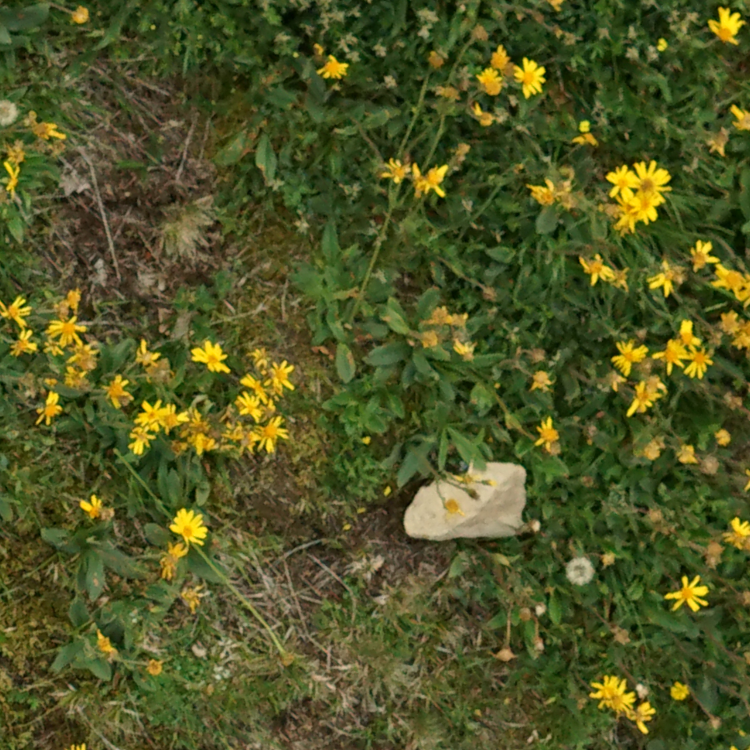
\includegraphics[width=0.24\textwidth]{abb/ergebnisse/gleicheblumen/DSC01525-b}}
    \subfigure[Flug 2]{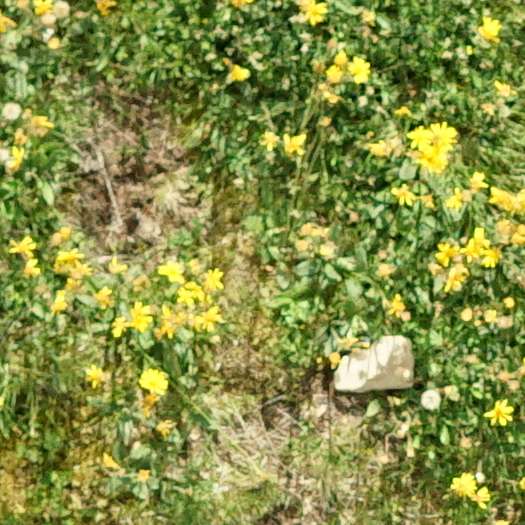
\includegraphics[width=0.24\textwidth]{abb/ergebnisse/gleicheblumen/DSC01298-b}}
    \subfigure[Flug 3]{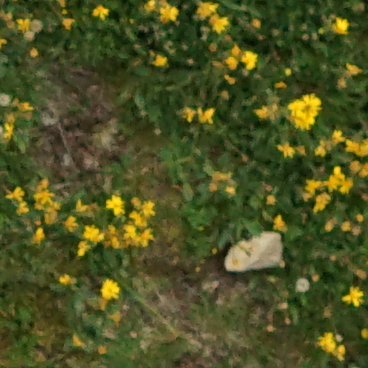
\includegraphics[width=0.24\textwidth]{abb/ergebnisse/gleicheblumen/DSC01757-b}}
    \subfigure[Flug 4]{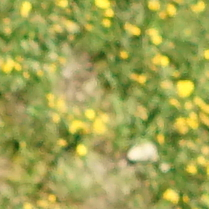
\includegraphics[width=0.24\textwidth]{abb/ergebnisse/gleicheblumen/DSC01959-b}}
\caption{Gleicher Bildausschnitt mit unterschiedlicher Auflösung je nach Flughöhe.}
  \label{fig:gleicheblumen}
\end{figure}

% Aufnahmenqualität bewerten
  %- unterschiedliche Lichtverhältnisse der Aufnahmen, Sonnenschein oder Schattenwurf 
  %- durch Bewegung unschärfe, vielleicht auch Belichtungszeit der Kamera nicht gut eingestellt?
  %- 
  
%   FLUGPLANUNG ??? UND ÜBERLAPPUNG DER BILDER -> ORTHOFOTO?

%++++++++++ wissenschaftlicher Kenntnissstand von Monitoring via Drohnen bzw. von automatischer Erkennung und Programmierung ???


%- die Testflüge dienten als erste Orientierung, um sich darauf vorbereiten zu können, heraus zu finden welches Equipment notwendig ist und mit den entstandenen Bildern die Softwareentwicklung anzustoßen, aber das ist ein langer Prozess, bis dies tatsächlich beeendet ist.

%Ich nehme mir jetzt diese Testdaten und teste wie mit "einfachen" mitteln das erreicht werden kann. 
% - Meine Software bietet die Möglichkeit sich einen Überblick zu verschaffen, für die qualitative Analyse nicht so geeignet.

% Testdaten sind Grundlage für mich zur Entwicklung des Programms und zur Bewertung der Funktion, 

